% --------------------------------------------------------------
% This is all preamble stuff that you don't have to worry about.
% Head down to where it says "Start here"
% --------------------------------------------------------------

\documentclass[12pt]{article}

\usepackage[margin=1in]{geometry}
\usepackage{amsmath,amsthm,amssymb}
\usepackage{graphicx} %This allows to include eps figures

% This is to include code
\usepackage{listings}
\usepackage{xcolor}
\usepackage{caption}
\usepackage{subcaption}
\definecolor{dkgreen}{rgb}{0,0.6,0}
\definecolor{gray}{rgb}{0.5,0.5,0.5}
\definecolor{mauve}{rgb}{0.58,0,0.82}
\lstdefinestyle{Python}{
    language        = Python,
    basicstyle      = \ttfamily,
    keywordstyle    = \color{blue},
    keywordstyle    = [2] \color{teal}, % just to check that it works
    stringstyle     = \color{green},
    commentstyle    = \color{red}\ttfamily
}

\newcommand{\N}{\mathbb{N}}
\newcommand{\Z}{\mathbb{Z}}

\newenvironment{theorem}[2][Theorem]{\begin{trivlist}
\item[\hskip \labelsep {\bfseries #1}\hskip \labelsep {\bfseries #2.}]}{\end{trivlist}}
\newenvironment{lemma}[2][Lemma]{\begin{trivlist}
\item[\hskip \labelsep {\bfseries #1}\hskip \labelsep {\bfseries #2.}]}{\end{trivlist}}
\newenvironment{exercise}[2][Exercise]{\begin{trivlist}
\item[\hskip \labelsep {\bfseries #1}\hskip \labelsep {\bfseries #2.}]}{\end{trivlist}}
\newenvironment{reflection}[2][Reflection]{\begin{trivlist}
\item[\hskip \labelsep {\bfseries #1}\hskip \labelsep {\bfseries #2.}]}{\end{trivlist}}
\newenvironment{proposition}[2][Proposition]{\begin{trivlist}
\item[\hskip \labelsep {\bfseries #1}\hskip \labelsep {\bfseries #2.}]}{\end{trivlist}}
\newenvironment{corollary}[2][Corollary]{\begin{trivlist}
\item[\hskip \labelsep {\bfseries #1}\hskip \labelsep {\bfseries #2.}]}{\end{trivlist}}

\begin{document}

% --------------------------------------------------------------
%                         Start here
% --------------------------------------------------------------

%\renewcommand{\qedsymbol}{\filledbox}

\title{Homework 3}%replace X with the appropriate number
\author{Thomas Buchegger\\ %replace with your name
Introduction to Signal and Image Processing}
\maketitle

\setcounter{tocdepth}3 % Set the depth of the table of contents to show sections and subsections only
\tableofcontents

\pagebreak
\section{Ransac}
\subsection{Introduction}
RANSAC (random sample consensus) is a rather simple algorithm designed to cope with a large proprtion of outliners in input data.
It is a resampling technique which generates different solutions by using the minimum number of data points required to estimate 
the underlying model parameters. Unlike other estimation techniques which use as much data as possible, RANSAC only uses the smallest 
possible set and proceeds to enlarge this set with consistent data points.
\newline

The algorithm can be broken down to 5 steps
\begin{enumerate}
    \item Select randomly minimum number of points to determine the model parameters
    \item Solve for the parameter of the model
    \item Determine how many points from the set of all points fit with a predefinded tolerance
    \item If fraction of number of inliners over the total number points in the set exceed a predefined threshold, re-estimate model parameters using all identified inliners and terminate
    \item Else, repeate steps 1 to 4 (N iterations)
\end{enumerate}

The number of iterations should be chosen high to ensure that at least one set of random samples does not include any outliners.

\pagebreak
\subsection{Results}
The following pictures are the results with the ransac algorithm. The used parameters are:
\begin{itemize}
    \item Iterations = 500
    \item Threshold = 2
    \item n samples = 2
    \end{itemize}

\begin{figure}[!htb]
    \centering
    %omit extension of file. pdflatex will convert to pdf automatically.
    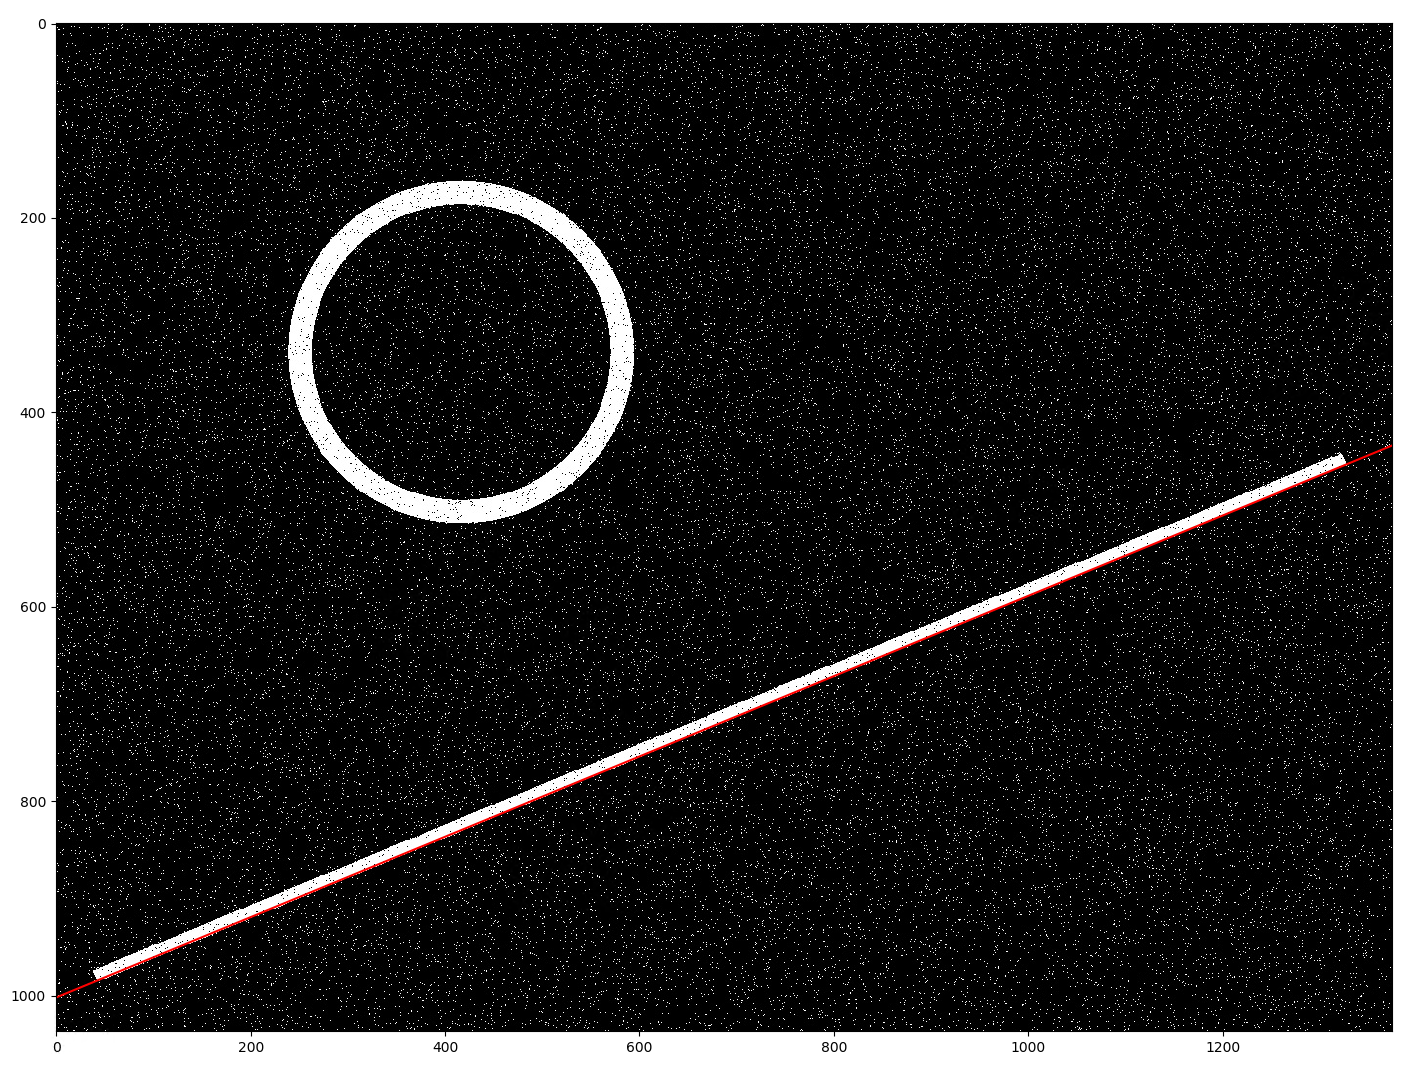
\includegraphics[width=0.5\textwidth]{pics/synthetic}
    \caption{Found line aligns well with the only line in the picture}
    \end{figure}

    \begin{figure}[!htb]
        \centering
        %omit extension of file. pdflatex will convert to pdf automatically.
        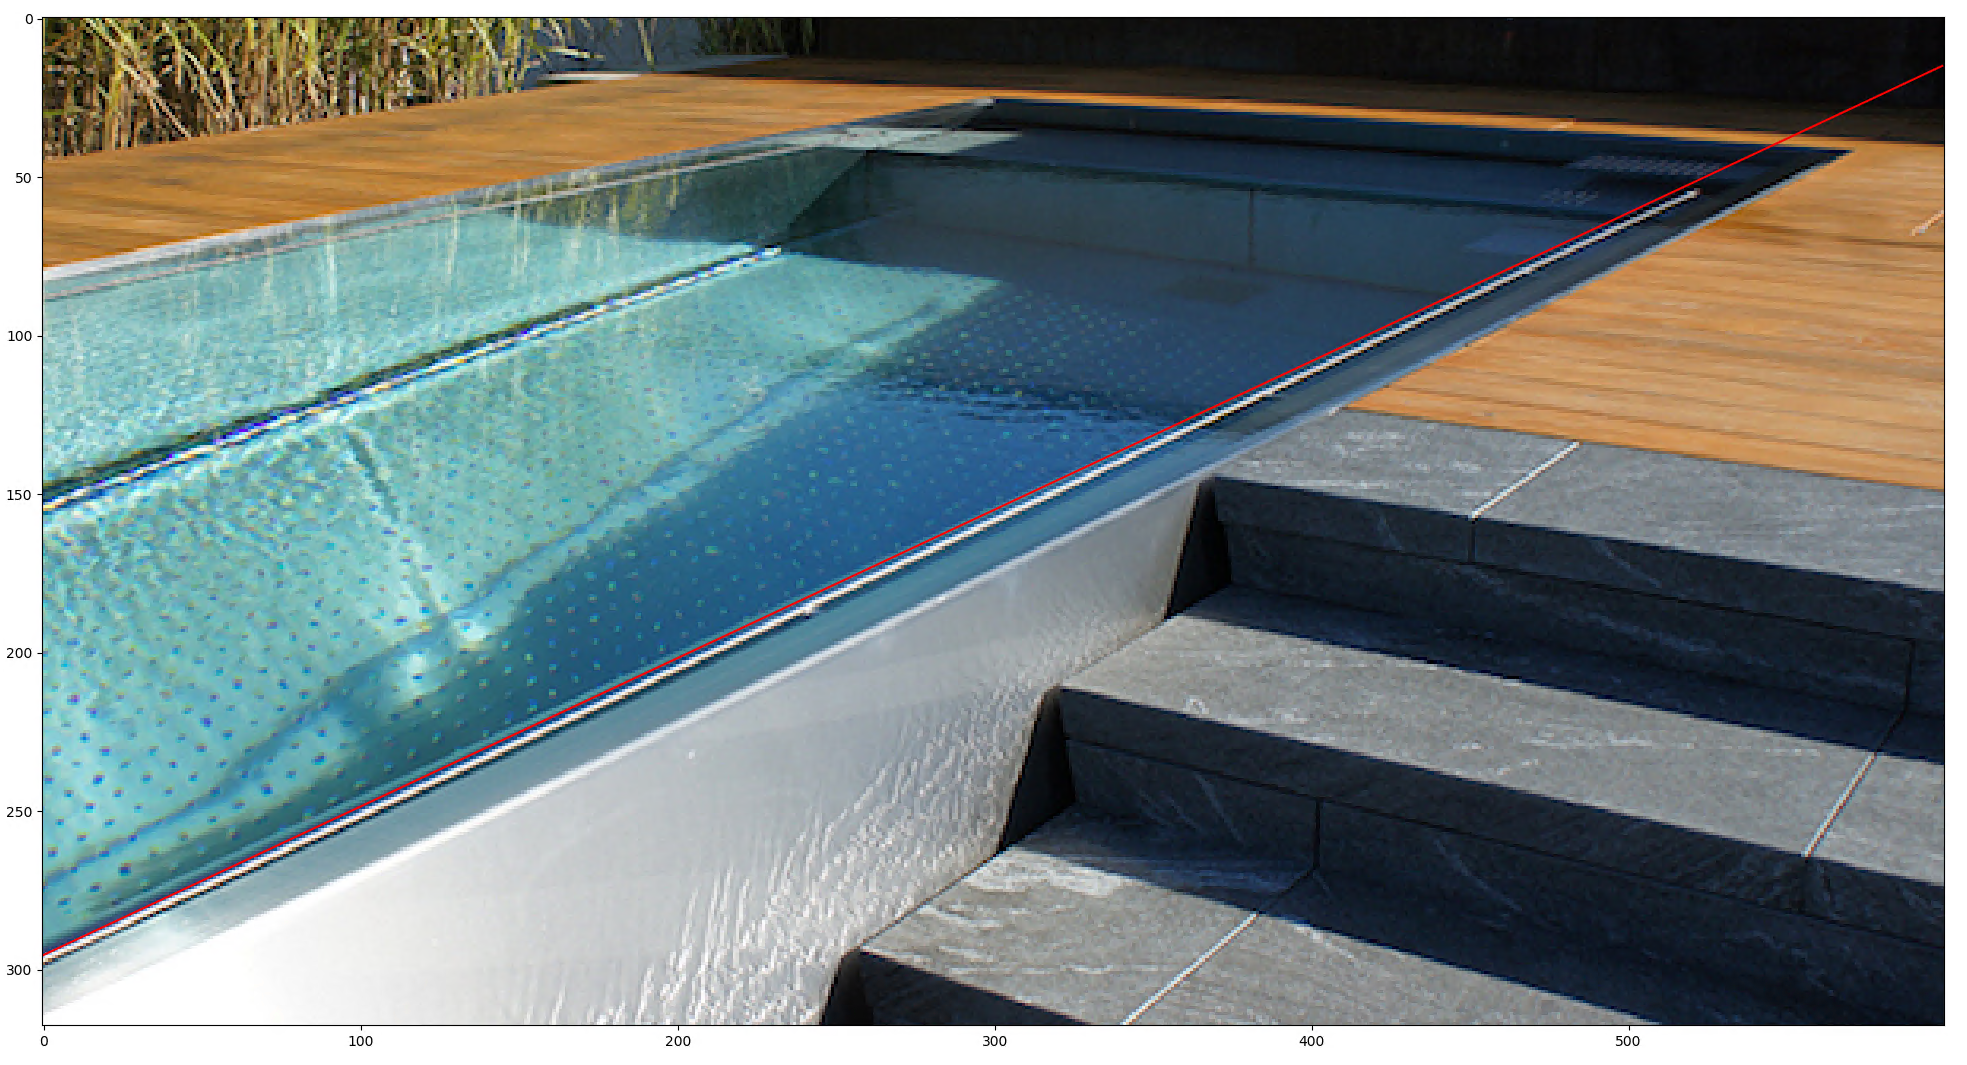
\includegraphics[width=0.5\textwidth]{pics/pool}
        \caption{Found line aligns with inner edge of pool}
        \end{figure}

\pagebreak

\begin{figure}[!htb]
    \centering
    %omit extension of file. pdflatex will convert to pdf automatically.
    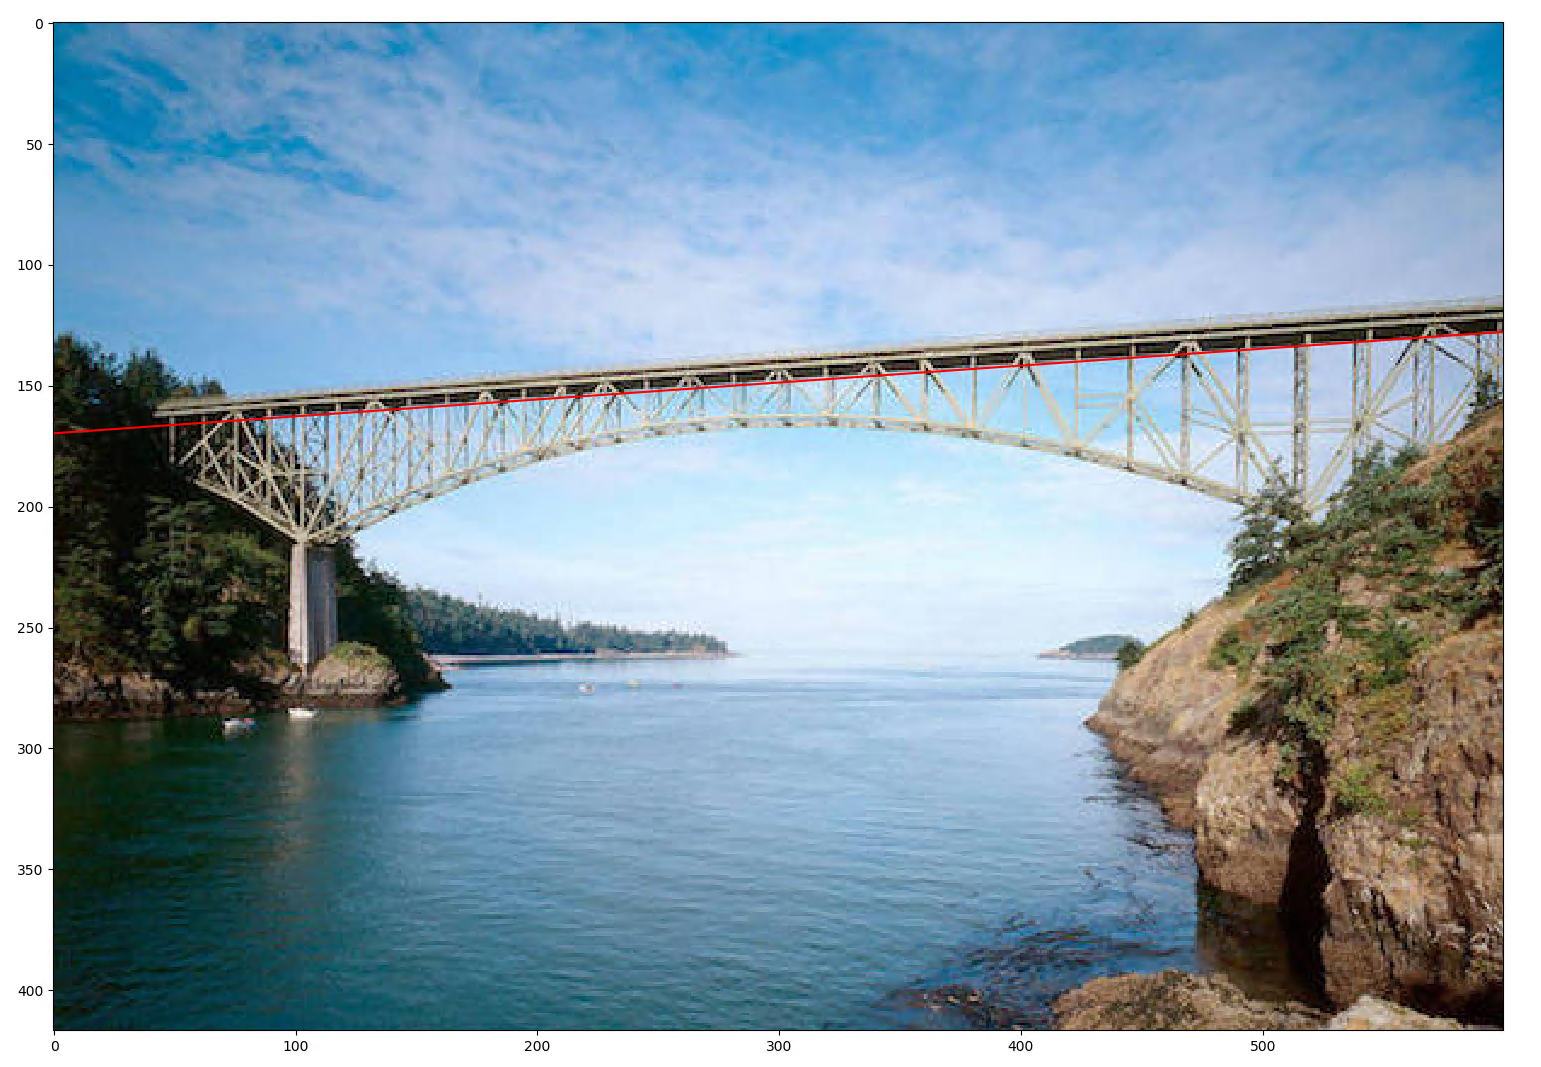
\includegraphics[width=0.5\textwidth]{pics/bridge}
    \caption{Found line aligns with bottom part of bridge}
    \end{figure}

\begin{figure}[!htb]
    \centering
    %omit extension of file. pdflatex will convert to pdf automatically.
    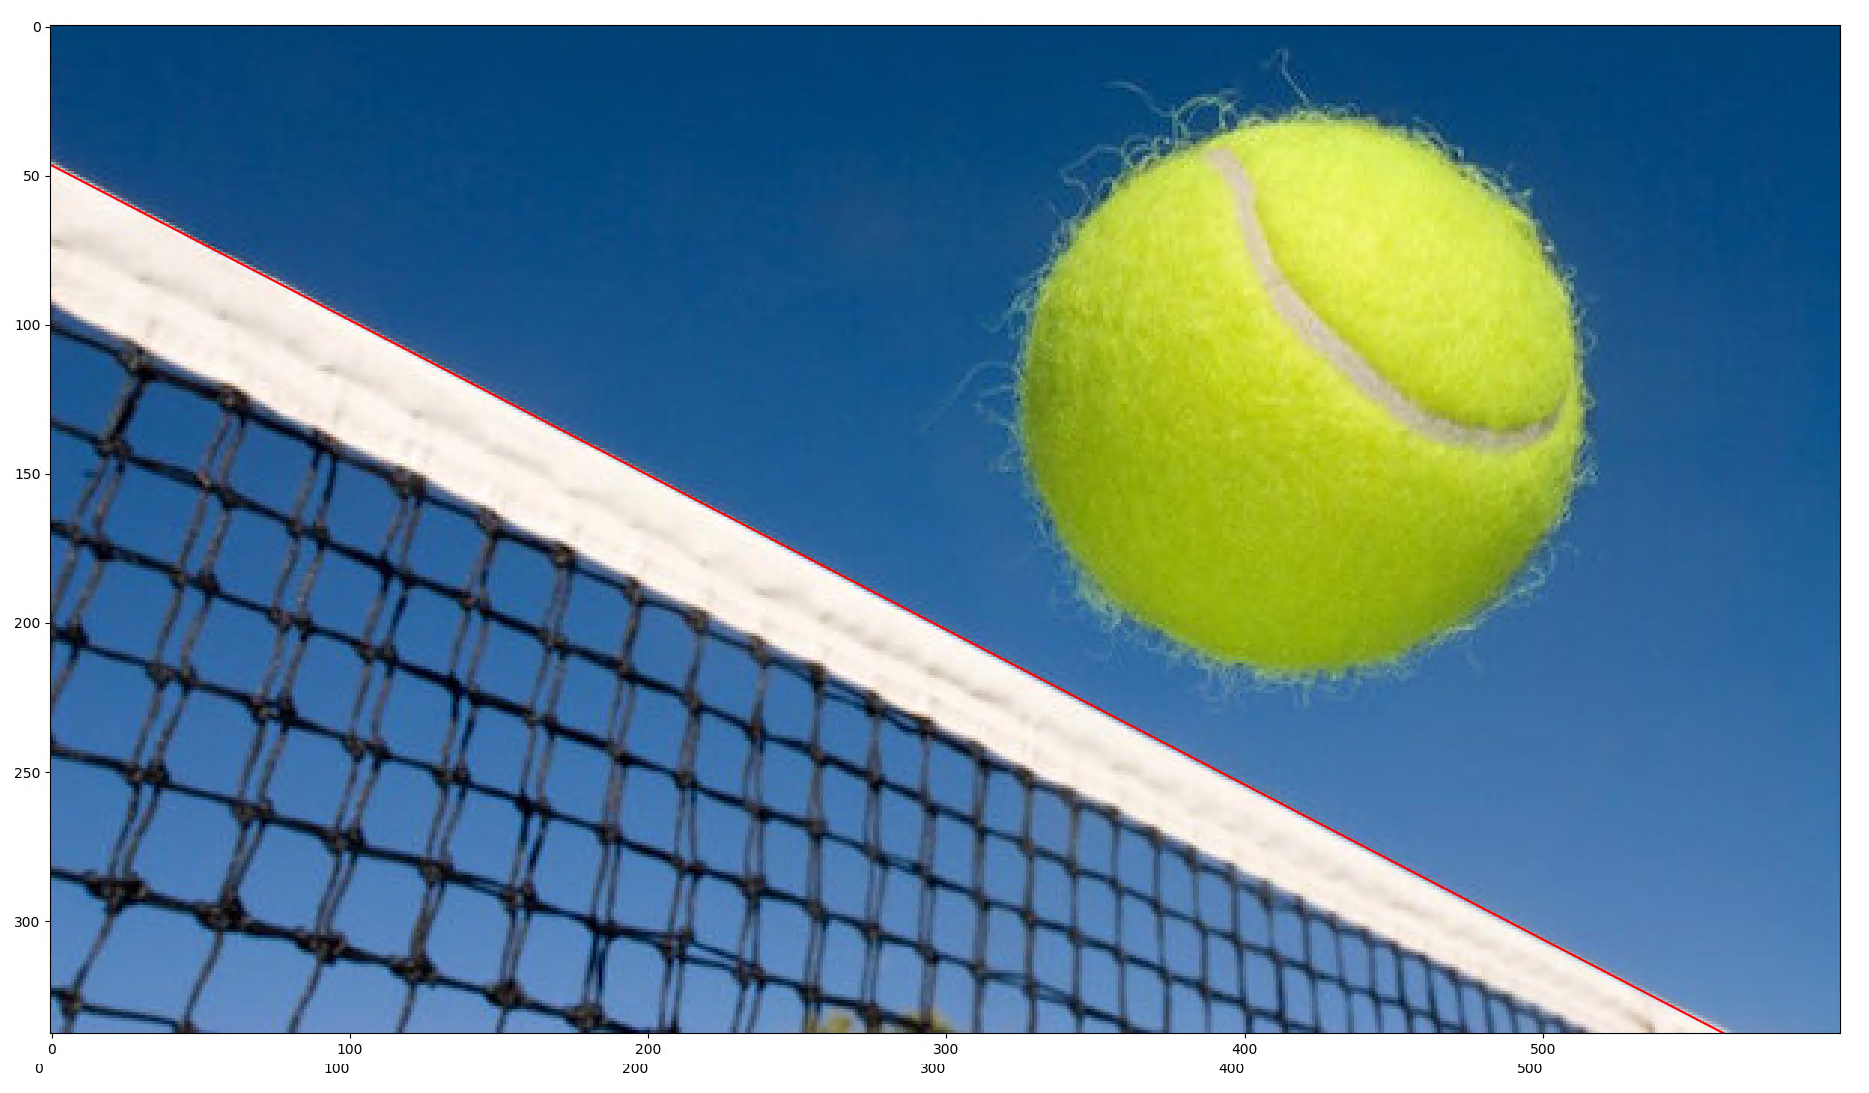
\includegraphics[width=0.5\textwidth]{pics/tennis}
    \caption{Found line aligns with upper edge of the net}
    \end{figure}

\pagebreak

\section{Texture Synthesis}
\subsection{Introduction}


\begin{figure}[!htb]
    \centering
    %omit extension of file. pdflatex will convert to pdf automatically.
    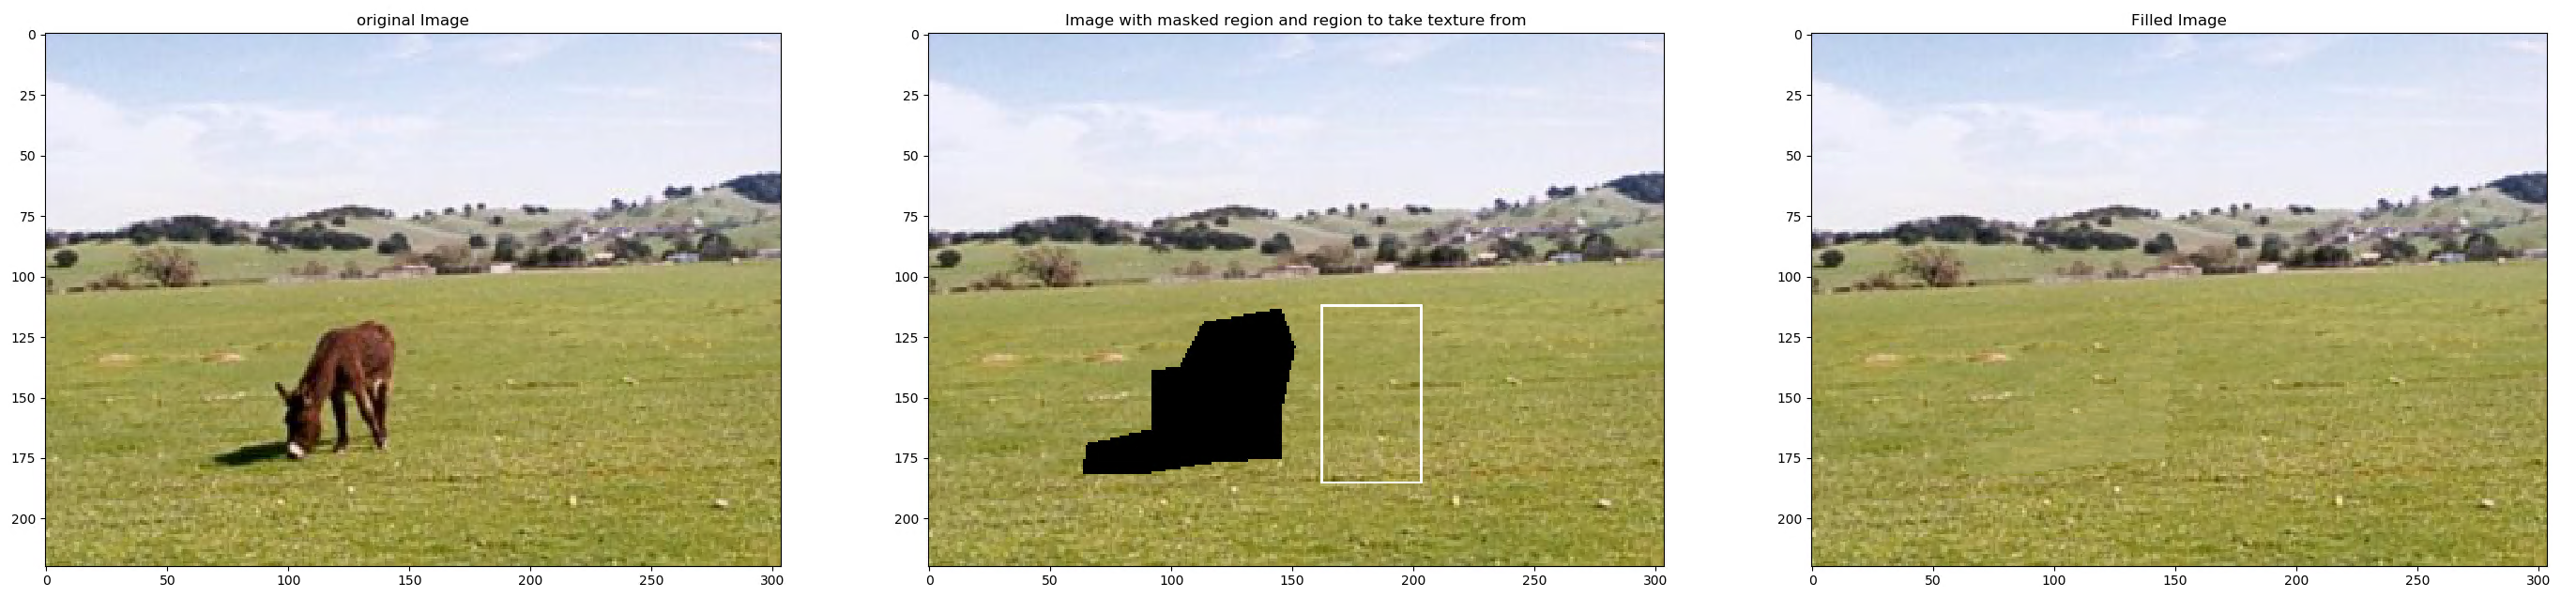
\includegraphics[width=0.8\textwidth]{pics/donkey10}
    \caption{With patch of size 10}
    \label{fig:boxfilter}
    \end{figure}

\end{document}